\documentclass[1p]{elsarticle_modified}
%\bibliographystyle{elsarticle-num}

%\usepackage[colorlinks]{hyperref}
%\usepackage{abbrmath_seonhwa} %\Abb, \Ascr, \Acal ,\Abf, \Afrak
\usepackage{amsfonts}
\usepackage{amssymb}
\usepackage{amsmath}
\usepackage{amsthm}
\usepackage{scalefnt}
\usepackage{amsbsy}
\usepackage{kotex}
\usepackage{caption}
\usepackage{subfig}
\usepackage{color}
\usepackage{graphicx}
\usepackage{xcolor} %% white, black, red, green, blue, cyan, magenta, yellow
\usepackage{float}
\usepackage{setspace}
\usepackage{hyperref}

\usepackage{tikz}
\usetikzlibrary{arrows}

\usepackage{multirow}
\usepackage{array} % fixed length table
\usepackage{hhline}

%%%%%%%%%%%%%%%%%%%%%
\makeatletter
\renewcommand*\env@matrix[1][\arraystretch]{%
	\edef\arraystretch{#1}%
	\hskip -\arraycolsep
	\let\@ifnextchar\new@ifnextchar
	\array{*\c@MaxMatrixCols c}}
\makeatother %https://tex.stackexchange.com/questions/14071/how-can-i-increase-the-line-spacing-in-a-matrix
%%%%%%%%%%%%%%%

\usepackage[normalem]{ulem}

\newcommand{\msout}[1]{\ifmmode\text{\sout{\ensuremath{#1}}}\else\sout{#1}\fi}
%SOURCE: \msout is \stkout macro in https://tex.stackexchange.com/questions/20609/strikeout-in-math-mode

\newcommand{\cancel}[1]{
	\ifmmode
	{\color{red}\msout{#1}}
	\else
	{\color{red}\sout{#1}}
	\fi
}

\newcommand{\add}[1]{
	{\color{blue}\uwave{#1}}
}

\newcommand{\replace}[2]{
	\ifmmode
	{\color{red}\msout{#1}}{\color{blue}\uwave{#2}}
	\else
	{\color{red}\sout{#1}}{\color{blue}\uwave{#2}}
	\fi
}

\newcommand{\Sol}{\mathcal{S}} %segment
\newcommand{\D}{D} %diagram
\newcommand{\A}{\mathcal{A}} %arc


%%%%%%%%%%%%%%%%%%%%%%%%%%%%%5 test

\def\sl{\operatorname{\textup{SL}}(2,\Cbb)}
\def\psl{\operatorname{\textup{PSL}}(2,\Cbb)}
\def\quan{\mkern 1mu \triangleright \mkern 1mu}

\theoremstyle{definition}
\newtheorem{thm}{Theorem}[section]
\newtheorem{prop}[thm]{Proposition}
\newtheorem{lem}[thm]{Lemma}
\newtheorem{ques}[thm]{Question}
\newtheorem{cor}[thm]{Corollary}
\newtheorem{defn}[thm]{Definition}
\newtheorem{exam}[thm]{Example}
\newtheorem{rmk}[thm]{Remark}
\newtheorem{alg}[thm]{Algorithm}

\newcommand{\I}{\sqrt{-1}}
\begin{document}

%\begin{frontmatter}
%
%\title{Boundary parabolic representations of knots up to 8 crossings}
%
%%% Group authors per affiliation:
%\author{Yunhi Cho} 
%\address{Department of Mathematics, University of Seoul, Seoul, Korea}
%\ead{yhcho@uos.ac.kr}
%
%
%\author{Seonhwa Kim} %\fnref{s_kim}}
%\address{Center for Geometry and Physics, Institute for Basic Science, Pohang, 37673, Korea}
%\ead{ryeona17@ibs.re.kr}
%
%\author{Hyuk Kim}
%\address{Department of Mathematical Sciences, Seoul National University, Seoul 08826, Korea}
%\ead{hyukkim@snu.ac.kr}
%
%\author{Seokbeom Yoon}
%\address{Department of Mathematical Sciences, Seoul National University, Seoul, 08826,  Korea}
%\ead{sbyoon15@snu.ac.kr}
%
%\begin{abstract}
%We find all boundary parabolic representation of knots up to 8 crossings.
%
%\end{abstract}
%\begin{keyword}
%    \MSC[2010] 57M25 
%\end{keyword}
%
%\end{frontmatter}

%\linenumbers
%\tableofcontents
%
\newcommand\colored[1]{\textcolor{white}{\rule[-0.35ex]{0.8em}{1.4ex}}\kern-0.8em\color{red} #1}%
%\newcommand\colored[1]{\textcolor{white}{ #1}\kern-2.17ex	\textcolor{white}{ #1}\kern-1.81ex	\textcolor{white}{ #1}\kern-2.15ex\color{red}#1	}

{\Large $\underline{12n_{0032}~(K12n_{0032})}$}

\setlength{\tabcolsep}{10pt}
\renewcommand{\arraystretch}{1.6}
\vspace{1cm}\begin{tabular}{m{100pt}>{\centering\arraybackslash}m{274pt}}
\multirow{5}{120pt}{
	\centering
	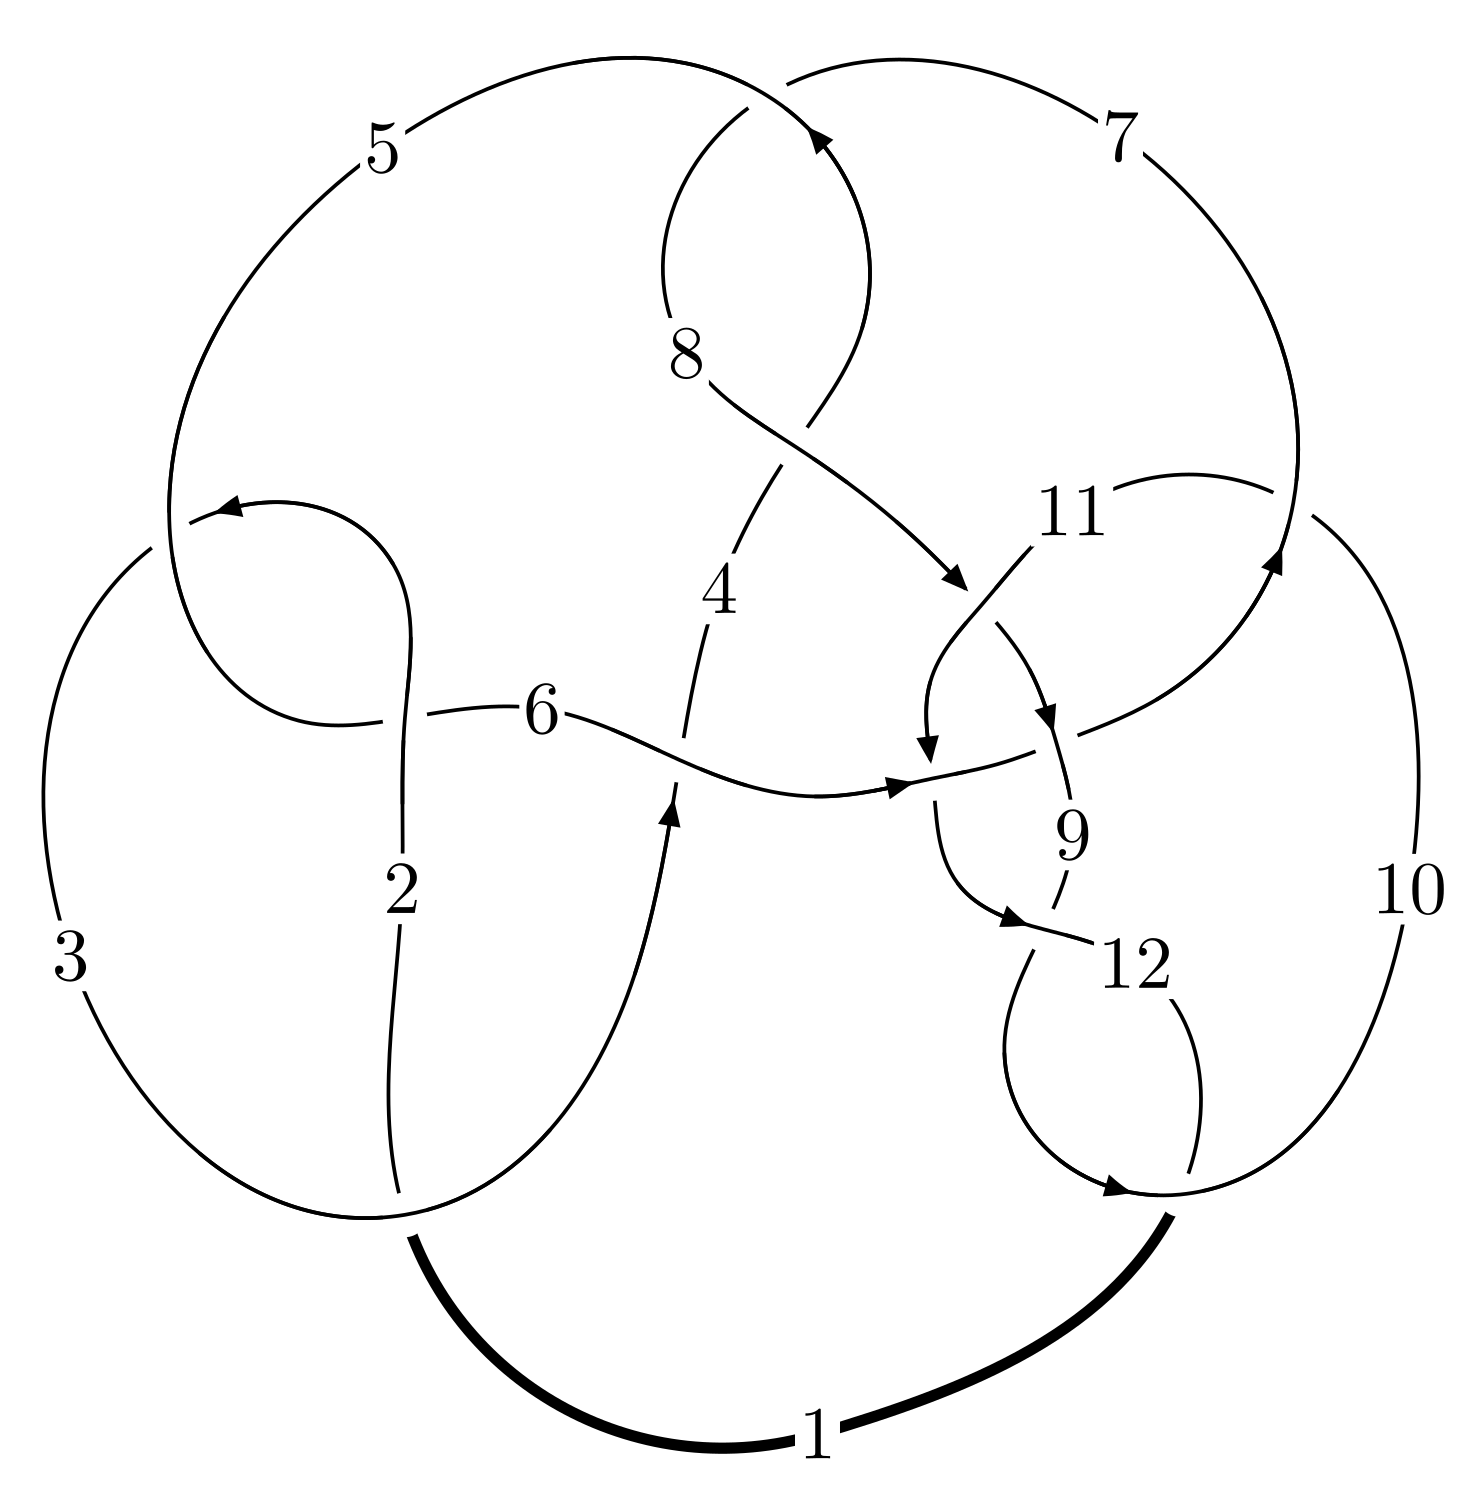
\includegraphics[width=112pt]{../../../GIT/diagram.site/Diagrams/png/2121_12n_0032.png}\\
\ \ \ A knot diagram\footnotemark}&
\allowdisplaybreaks
\textbf{Linearized knot diagam} \\
\cline{2-2}
 &
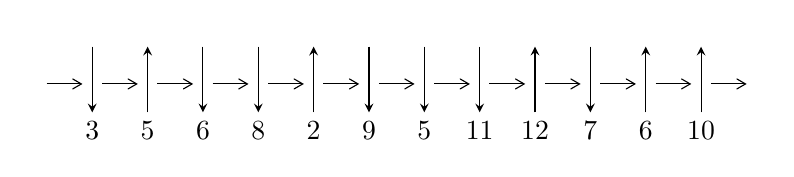
\begin{tikzpicture}[x=20pt, y=17pt]
	% nodes
	\node (C0) at (0, 0) {};
	\node (C1) at (1, 0) {};
	\node (C1U) at (1, +1) {};
	\node (C1D) at (1, -1) {3};

	\node (C2) at (2, 0) {};
	\node (C2U) at (2, +1) {};
	\node (C2D) at (2, -1) {5};

	\node (C3) at (3, 0) {};
	\node (C3U) at (3, +1) {};
	\node (C3D) at (3, -1) {6};

	\node (C4) at (4, 0) {};
	\node (C4U) at (4, +1) {};
	\node (C4D) at (4, -1) {8};

	\node (C5) at (5, 0) {};
	\node (C5U) at (5, +1) {};
	\node (C5D) at (5, -1) {2};

	\node (C6) at (6, 0) {};
	\node (C6U) at (6, +1) {};
	\node (C6D) at (6, -1) {9};

	\node (C7) at (7, 0) {};
	\node (C7U) at (7, +1) {};
	\node (C7D) at (7, -1) {5};

	\node (C8) at (8, 0) {};
	\node (C8U) at (8, +1) {};
	\node (C8D) at (8, -1) {11};

	\node (C9) at (9, 0) {};
	\node (C9U) at (9, +1) {};
	\node (C9D) at (9, -1) {12};

	\node (C10) at (10, 0) {};
	\node (C10U) at (10, +1) {};
	\node (C10D) at (10, -1) {7};

	\node (C11) at (11, 0) {};
	\node (C11U) at (11, +1) {};
	\node (C11D) at (11, -1) {6};

	\node (C12) at (12, 0) {};
	\node (C12U) at (12, +1) {};
	\node (C12D) at (12, -1) {10};
	\node (C13) at (13, 0) {};

	% arrows
	\draw[->,>={angle 60}]
	(C0) edge (C1) (C1) edge (C2) (C2) edge (C3) (C3) edge (C4) (C4) edge (C5) (C5) edge (C6) (C6) edge (C7) (C7) edge (C8) (C8) edge (C9) (C9) edge (C10) (C10) edge (C11) (C11) edge (C12) (C12) edge (C13) ;	\draw[->,>=stealth]
	(C1U) edge (C1D) (C2D) edge (C2U) (C3U) edge (C3D) (C4U) edge (C4D) (C5D) edge (C5U) (C6U) edge (C6D) (C7U) edge (C7D) (C8U) edge (C8D) (C9D) edge (C9U) (C10U) edge (C10D) (C11D) edge (C11U) (C12D) edge (C12U) ;
	\end{tikzpicture} \\
\hhline{~~} \\& 
\textbf{Solving Sequence} \\ \cline{2-2} 
 &
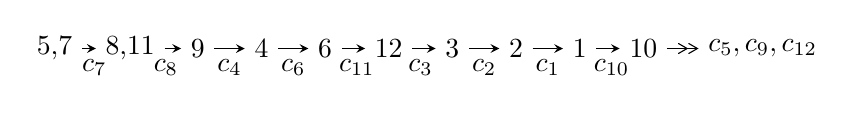
\begin{tikzpicture}[x=23pt, y=7pt]
	% node
	\node (A0) at (-1/8, 0) {5,7};
	\node (A1) at (17/16, 0) {8,11};
	\node (A2) at (17/8, 0) {9};
	\node (A3) at (25/8, 0) {4};
	\node (A4) at (33/8, 0) {6};
	\node (A5) at (41/8, 0) {12};
	\node (A6) at (49/8, 0) {3};
	\node (A7) at (57/8, 0) {2};
	\node (A8) at (65/8, 0) {1};
	\node (A9) at (73/8, 0) {10};
	\node (C1) at (1/2, -1) {$c_{7}$};
	\node (C2) at (13/8, -1) {$c_{8}$};
	\node (C3) at (21/8, -1) {$c_{4}$};
	\node (C4) at (29/8, -1) {$c_{6}$};
	\node (C5) at (37/8, -1) {$c_{11}$};
	\node (C6) at (45/8, -1) {$c_{3}$};
	\node (C7) at (53/8, -1) {$c_{2}$};
	\node (C8) at (61/8, -1) {$c_{1}$};
	\node (C9) at (69/8, -1) {$c_{10}$};
	\node (A10) at (11, 0) {$c_{5},c_{9},c_{12}$};

	% edge
	\draw[->,>=stealth]	
	(A0) edge (A1) (A1) edge (A2) (A2) edge (A3) (A3) edge (A4) (A4) edge (A5) (A5) edge (A6) (A6) edge (A7) (A7) edge (A8) (A8) edge (A9) ;
	\draw[->>,>={angle 60}]	
	(A9) edge (A10);
\end{tikzpicture} \\ 

\end{tabular} \\

\footnotetext{
The image of knot diagram is generated by the software ``\textbf{Draw programme}" developed by Andrew Bartholomew(\url{http://www.layer8.co.uk/maths/draw/index.htm\#Running-draw}), where we modified some parts for our purpose(\url{https://github.com/CATsTAILs/LinksPainter}).
}\phantom \\ \newline 
\centering \textbf{Ideals for irreducible components\footnotemark of $X_{\text{par}}$} 
 
\begin{align*}
I^u_{1}&=\langle 
-4.78378\times10^{254} u^{64}+1.08998\times10^{255} u^{63}+\cdots+3.15176\times10^{257} b-2.19432\times10^{258},\\
\phantom{I^u_{1}}&\phantom{= \langle  }3.69307\times10^{254} u^{64}+2.76585\times10^{254} u^{63}+\cdots+6.30351\times10^{257} a+1.47988\times10^{259},\\
\phantom{I^u_{1}}&\phantom{= \langle  }u^{65}-2 u^{64}+\cdots+4096 u+4096\rangle \\
I^u_{2}&=\langle 
- u^4+2 u^3+u^2+b-3 u,\;3 u^4-3 u^3-7 u^2+a+5 u+4,\;u^5- u^4-2 u^3+u^2+u+1\rangle \\
\\
I^v_{1}&=\langle 
a,\;164522 v^{11}-355934 v^{10}+\cdots+707733 b+176501,\\
\phantom{I^v_{1}}&\phantom{= \langle  }v^{12}-3 v^{11}+3 v^{10}-18 v^9+31 v^8+29 v^7-31 v^6+9 v^5+19 v^4-5 v^3-4 v^2- v+1\rangle \\
\end{align*}
\raggedright * 3 irreducible components of $\dim_{\mathbb{C}}=0$, with total 82 representations.\\
\footnotetext{All coefficients of polynomials are rational numbers. But the coefficients are sometimes approximated in decimal forms when there is not enough margin.}
\newpage
\renewcommand{\arraystretch}{1}
\centering \section*{I. $I^u_{1}= \langle -4.78\times10^{254} u^{64}+1.09\times10^{255} u^{63}+\cdots+3.15\times10^{257} b-2.19\times10^{258},\;3.69\times10^{254} u^{64}+2.77\times10^{254} u^{63}+\cdots+6.30\times10^{257} a+1.48\times10^{259},\;u^{65}-2 u^{64}+\cdots+4096 u+4096 \rangle$}
\flushleft \textbf{(i) Arc colorings}\\
\begin{tabular}{m{7pt} m{180pt} m{7pt} m{180pt} }
\flushright $a_{5}=$&$\begin{pmatrix}0\\u\end{pmatrix}$ \\
\flushright $a_{7}=$&$\begin{pmatrix}1\\0\end{pmatrix}$ \\
\flushright $a_{8}=$&$\begin{pmatrix}1\\u^2\end{pmatrix}$ \\
\flushright $a_{11}=$&$\begin{pmatrix}-0.000585875 u^{64}-0.000438779 u^{63}+\cdots+20.3734 u-23.4770\\0.00151782 u^{64}-0.00345832 u^{63}+\cdots+9.59064 u+6.96221\end{pmatrix}$ \\
\flushright $a_{9}=$&$\begin{pmatrix}-0.0000458644 u^{64}-0.000173442 u^{63}+\cdots+1.67151 u-5.60504\\0.0000363689 u^{64}-0.000165732 u^{63}+\cdots+2.08385 u-0.210615\end{pmatrix}$ \\
\flushright $a_{4}=$&$\begin{pmatrix}u\\u^3+u\end{pmatrix}$ \\
\flushright $a_{6}=$&$\begin{pmatrix}0.000476569 u^{64}-0.000749697 u^{63}+\cdots+3.33404 u+5.48921\\-0.0000745146 u^{64}+0.000168353 u^{63}+\cdots-0.709852 u-0.337516\end{pmatrix}$ \\
\flushright $a_{12}=$&$\begin{pmatrix}0.00116546 u^{64}-0.00414819 u^{63}+\cdots+31.2869 u-11.0123\\0.00138687 u^{64}-0.00313302 u^{63}+\cdots+8.32770 u+7.09279\end{pmatrix}$ \\
\flushright $a_{3}=$&$\begin{pmatrix}-0.000390199 u^{64}+0.000564940 u^{63}+\cdots-0.279557 u-4.94851\\0.000137437 u^{64}-0.000304135 u^{63}+\cdots+2.61125 u+0.546810\end{pmatrix}$ \\
\flushright $a_{2}=$&$\begin{pmatrix}-0.000390199 u^{64}+0.000564940 u^{63}+\cdots-0.279557 u-4.94851\\0.000398870 u^{64}-0.000884646 u^{63}+\cdots+5.09202 u+1.42933\end{pmatrix}$ \\
\flushright $a_{1}=$&$\begin{pmatrix}-0.000327023 u^{64}+0.000433323 u^{63}+\cdots-1.25857 u-4.99343\\0.000149546 u^{64}-0.000316374 u^{63}+\cdots+2.07547 u+0.495780\end{pmatrix}$ \\
\flushright $a_{10}=$&$\begin{pmatrix}0.000931941 u^{64}-0.00389710 u^{63}+\cdots+29.9641 u-16.5148\\0.00151782 u^{64}-0.00345832 u^{63}+\cdots+9.59064 u+6.96221\end{pmatrix}$\\&\end{tabular}
\flushleft \textbf{(ii) Obstruction class $= -1$}\\~\\
\flushleft \textbf{(iii) Cusp Shapes $= 0.0401453 u^{64}-0.0971031 u^{63}+\cdots+376.505 u+118.641$}\\~\\
\newpage\renewcommand{\arraystretch}{1}
\flushleft \textbf{(iv) u-Polynomials at the component}\newline \\
\begin{tabular}{m{50pt}|m{274pt}}
Crossings & \hspace{64pt}u-Polynomials at each crossing \\
\hline $$\begin{aligned}c_{1}\end{aligned}$$&$\begin{aligned}
&u^{65}+18 u^{64}+\cdots-47 u-1
\end{aligned}$\\
\hline $$\begin{aligned}c_{2},c_{5}\end{aligned}$$&$\begin{aligned}
&u^{65}+8 u^{64}+\cdots+5 u+1
\end{aligned}$\\
\hline $$\begin{aligned}c_{3}\end{aligned}$$&$\begin{aligned}
&u^{65}-8 u^{64}+\cdots+103537045 u+13657673
\end{aligned}$\\
\hline $$\begin{aligned}c_{4},c_{7}\end{aligned}$$&$\begin{aligned}
&u^{65}-2 u^{64}+\cdots+4096 u+4096
\end{aligned}$\\
\hline $$\begin{aligned}c_{6}\end{aligned}$$&$\begin{aligned}
&u^{65}-4 u^{64}+\cdots-3 u+1
\end{aligned}$\\
\hline $$\begin{aligned}c_{8}\end{aligned}$$&$\begin{aligned}
&u^{65}-11 u^{64}+\cdots-192 u+32
\end{aligned}$\\
\hline $$\begin{aligned}c_{9},c_{12}\end{aligned}$$&$\begin{aligned}
&u^{65}+8 u^{64}+\cdots+3 u+1
\end{aligned}$\\
\hline $$\begin{aligned}c_{10}\end{aligned}$$&$\begin{aligned}
&u^{65}+4 u^{64}+\cdots-606921 u+85049
\end{aligned}$\\
\hline $$\begin{aligned}c_{11}\end{aligned}$$&$\begin{aligned}
&u^{65}+10 u^{64}+\cdots+497 u+101
\end{aligned}$\\
\hline
\end{tabular}\\~\\
\newpage\renewcommand{\arraystretch}{1}
\flushleft \textbf{(v) Riley Polynomials at the component}\newline \\
\begin{tabular}{m{50pt}|m{274pt}}
Crossings & \hspace{64pt}Riley Polynomials at each crossing \\
\hline $$\begin{aligned}c_{1}\end{aligned}$$&$\begin{aligned}
&y^{65}+66 y^{64}+\cdots+213 y-1
\end{aligned}$\\
\hline $$\begin{aligned}c_{2},c_{5}\end{aligned}$$&$\begin{aligned}
&y^{65}+18 y^{64}+\cdots-47 y-1
\end{aligned}$\\
\hline $$\begin{aligned}c_{3}\end{aligned}$$&$\begin{aligned}
&y^{65}+114 y^{64}+\cdots-13102594991519615 y-186532031774929
\end{aligned}$\\
\hline $$\begin{aligned}c_{4},c_{7}\end{aligned}$$&$\begin{aligned}
&y^{65}+60 y^{64}+\cdots-134217728 y-16777216
\end{aligned}$\\
\hline $$\begin{aligned}c_{6}\end{aligned}$$&$\begin{aligned}
&y^{65}+2 y^{64}+\cdots-19 y-1
\end{aligned}$\\
\hline $$\begin{aligned}c_{8}\end{aligned}$$&$\begin{aligned}
&y^{65}+27 y^{64}+\cdots-52736 y-1024
\end{aligned}$\\
\hline $$\begin{aligned}c_{9},c_{12}\end{aligned}$$&$\begin{aligned}
&y^{65}-58 y^{64}+\cdots-4257 y-1
\end{aligned}$\\
\hline $$\begin{aligned}c_{10}\end{aligned}$$&$\begin{aligned}
&y^{65}+4 y^{64}+\cdots+132226628699 y-7233332401
\end{aligned}$\\
\hline $$\begin{aligned}c_{11}\end{aligned}$$&$\begin{aligned}
&y^{65}-72 y^{64}+\cdots+1225295 y-10201
\end{aligned}$\\
\hline
\end{tabular}\\~\\
\newpage\flushleft \textbf{(vi) Complex Volumes and Cusp Shapes}
$$\begin{array}{c|c|c}  
\text{Solutions to }I^u_{1}& \I (\text{vol} + \sqrt{-1}CS) & \text{Cusp shape}\\
 \hline 
\begin{aligned}
u &= \phantom{-}0.130385 + 0.943634 I \\
a &= \phantom{-}0.76665 + 2.06572 I \\
b &= -0.514674 - 0.553942 I\end{aligned}
 & -0.74329 - 4.73729 I & -2.00000 + 8.64739 I \\ \hline\begin{aligned}
u &= \phantom{-}0.130385 - 0.943634 I \\
a &= \phantom{-}0.76665 - 2.06572 I \\
b &= -0.514674 + 0.553942 I\end{aligned}
 & -0.74329 + 4.73729 I & -2.00000 - 8.64739 I \\ \hline\begin{aligned}
u &= \phantom{-}0.887268 + 0.125733 I \\
a &= -0.179409 - 1.032200 I \\
b &= \phantom{-}0.318940 + 0.297442 I\end{aligned}
 & \phantom{-}1.48232 - 4.00344 I & -0.95634 + 8.48185 I \\ \hline\begin{aligned}
u &= \phantom{-}0.887268 - 0.125733 I \\
a &= -0.179409 + 1.032200 I \\
b &= \phantom{-}0.318940 - 0.297442 I\end{aligned}
 & \phantom{-}1.48232 + 4.00344 I & -0.95634 - 8.48185 I \\ \hline\begin{aligned}
u &= \phantom{-}0.668516 + 0.588632 I \\
a &= \phantom{-}1.56956 - 1.46497 I \\
b &= \phantom{-}0.016939 + 1.169930 I\end{aligned}
 & \phantom{-}3.65615 - 1.42936 I & \phantom{-}6.46603 + 3.32743 I \\ \hline\begin{aligned}
u &= \phantom{-}0.668516 - 0.588632 I \\
a &= \phantom{-}1.56956 + 1.46497 I \\
b &= \phantom{-}0.016939 - 1.169930 I\end{aligned}
 & \phantom{-}3.65615 + 1.42936 I & \phantom{-}6.46603 - 3.32743 I \\ \hline\begin{aligned}
u &= -0.802999\phantom{ +0.000000I} \\
a &= \phantom{-}0.258328\phantom{ +0.000000I} \\
b &= \phantom{-}0.781641\phantom{ +0.000000I}\end{aligned}
 & -1.43422\phantom{ +0.000000I} & -8.16770\phantom{ +0.000000I} \\ \hline\begin{aligned}
u &= \phantom{-}0.243832 + 0.761247 I \\
a &= \phantom{-}1.34826 - 1.30971 I \\
b &= -0.250649 + 0.069598 I\end{aligned}
 & \phantom{-}1.88543 + 1.32823 I & \phantom{-}3.63769 - 3.79947 I \\ \hline\begin{aligned}
u &= \phantom{-}0.243832 - 0.761247 I \\
a &= \phantom{-}1.34826 + 1.30971 I \\
b &= -0.250649 - 0.069598 I\end{aligned}
 & \phantom{-}1.88543 - 1.32823 I & \phantom{-}3.63769 + 3.79947 I \\ \hline\begin{aligned}
u &= -0.607968 + 0.481302 I \\
a &= \phantom{-}0.149356 + 0.154741 I \\
b &= \phantom{-}1.044290 - 0.031607 I\end{aligned}
 & -1.68242 - 0.00290 I & -4.75043 - 0.81603 I\\
 \hline 
 \end{array}$$\newpage$$\begin{array}{c|c|c}  
\text{Solutions to }I^u_{1}& \I (\text{vol} + \sqrt{-1}CS) & \text{Cusp shape}\\
 \hline 
\begin{aligned}
u &= -0.607968 - 0.481302 I \\
a &= \phantom{-}0.149356 - 0.154741 I \\
b &= \phantom{-}1.044290 + 0.031607 I\end{aligned}
 & -1.68242 + 0.00290 I & -4.75043 + 0.81603 I \\ \hline\begin{aligned}
u &= -0.031117 + 0.710250 I \\
a &= \phantom{-}1.88874 + 1.21810 I \\
b &= -0.608662 - 0.271807 I\end{aligned}
 & -0.54684 + 1.46329 I & -1.59201 - 1.40388 I \\ \hline\begin{aligned}
u &= -0.031117 - 0.710250 I \\
a &= \phantom{-}1.88874 - 1.21810 I \\
b &= -0.608662 + 0.271807 I\end{aligned}
 & -0.54684 - 1.46329 I & -1.59201 + 1.40388 I \\ \hline\begin{aligned}
u &= -0.704902 + 0.035674 I \\
a &= \phantom{-}1.00315 + 1.49097 I \\
b &= \phantom{-}0.615020 - 0.093383 I\end{aligned}
 & \phantom{-}1.30008 - 0.99581 I & -3.39411 - 0.67872 I \\ \hline\begin{aligned}
u &= -0.704902 - 0.035674 I \\
a &= \phantom{-}1.00315 - 1.49097 I \\
b &= \phantom{-}0.615020 + 0.093383 I\end{aligned}
 & \phantom{-}1.30008 + 0.99581 I & -3.39411 + 0.67872 I \\ \hline\begin{aligned}
u &= \phantom{-}0.536940 + 0.442415 I \\
a &= \phantom{-}0.096152 + 0.318851 I \\
b &= \phantom{-}0.948518 - 0.522416 I\end{aligned}
 & -2.50902 + 1.89252 I & -7.42573 - 0.50006 I \\ \hline\begin{aligned}
u &= \phantom{-}0.536940 - 0.442415 I \\
a &= \phantom{-}0.096152 - 0.318851 I \\
b &= \phantom{-}0.948518 + 0.522416 I\end{aligned}
 & -2.50902 - 1.89252 I & -7.42573 + 0.50006 I \\ \hline\begin{aligned}
u &= -0.423794 + 0.531866 I \\
a &= \phantom{-}1.09298 - 3.83683 I \\
b &= -1.83672 - 0.52554 I\end{aligned}
 & \phantom{-}1.19925 + 1.20786 I & \phantom{-}13.02298 - 5.31257 I \\ \hline\begin{aligned}
u &= -0.423794 - 0.531866 I \\
a &= \phantom{-}1.09298 + 3.83683 I \\
b &= -1.83672 + 0.52554 I\end{aligned}
 & \phantom{-}1.19925 - 1.20786 I & \phantom{-}13.02298 + 5.31257 I \\ \hline\begin{aligned}
u &= -0.584385 + 0.334144 I \\
a &= \phantom{-}0.118976 + 0.116953 I \\
b &= -0.863516 + 0.470481 I\end{aligned}
 & -0.48772 + 4.09297 I & -7.37755 - 9.24327 I\\
 \hline 
 \end{array}$$\newpage$$\begin{array}{c|c|c}  
\text{Solutions to }I^u_{1}& \I (\text{vol} + \sqrt{-1}CS) & \text{Cusp shape}\\
 \hline 
\begin{aligned}
u &= -0.584385 - 0.334144 I \\
a &= \phantom{-}0.118976 - 0.116953 I \\
b &= -0.863516 - 0.470481 I\end{aligned}
 & -0.48772 - 4.09297 I & -7.37755 + 9.24327 I \\ \hline\begin{aligned}
u &= -0.340196 + 0.558280 I \\
a &= \phantom{-}0.987313 + 0.431504 I \\
b &= -0.136703 - 0.358878 I\end{aligned}
 & -0.33530 + 1.50733 I & -2.98038 - 4.24113 I \\ \hline\begin{aligned}
u &= -0.340196 - 0.558280 I \\
a &= \phantom{-}0.987313 - 0.431504 I \\
b &= -0.136703 + 0.358878 I\end{aligned}
 & -0.33530 - 1.50733 I & -2.98038 + 4.24113 I \\ \hline\begin{aligned}
u &= \phantom{-}0.462414 + 0.447292 I \\
a &= \phantom{-}0.117142 + 0.093138 I \\
b &= -1.175610 + 0.714758 I\end{aligned}
 & \phantom{-}0.05754 + 7.13285 I & -1.292669 + 0.043034 I \\ \hline\begin{aligned}
u &= \phantom{-}0.462414 - 0.447292 I \\
a &= \phantom{-}0.117142 - 0.093138 I \\
b &= -1.175610 - 0.714758 I\end{aligned}
 & \phantom{-}0.05754 - 7.13285 I & -1.292669 - 0.043034 I \\ \hline\begin{aligned}
u &= -0.237497 + 0.569452 I \\
a &= \phantom{-}0.98989 + 4.44821 I \\
b &= \phantom{-}0.067363 - 1.017050 I\end{aligned}
 & \phantom{-}2.38609 - 2.85839 I & \phantom{-}7.30042 - 0.29630 I \\ \hline\begin{aligned}
u &= -0.237497 - 0.569452 I \\
a &= \phantom{-}0.98989 - 4.44821 I \\
b &= \phantom{-}0.067363 + 1.017050 I\end{aligned}
 & \phantom{-}2.38609 + 2.85839 I & \phantom{-}7.30042 + 0.29630 I \\ \hline\begin{aligned}
u &= \phantom{-}1.356580 + 0.325626 I \\
a &= \phantom{-}0.0929425 - 0.0475878 I \\
b &= \phantom{-}0.601262 - 0.221151 I\end{aligned}
 & -4.31980 - 4.20818 I & \phantom{-0.000000 } 0 \\ \hline\begin{aligned}
u &= \phantom{-}1.356580 - 0.325626 I \\
a &= \phantom{-}0.0929425 + 0.0475878 I \\
b &= \phantom{-}0.601262 + 0.221151 I\end{aligned}
 & -4.31980 + 4.20818 I & \phantom{-0.000000 } 0 \\ \hline\begin{aligned}
u &= -0.324505 + 0.474102 I \\
a &= \phantom{-}2.11235 + 9.22641 I \\
b &= \phantom{-}2.59859 - 1.54012 I\end{aligned}
 & \phantom{-}1.37708 + 1.55327 I & \phantom{-}81.0765 + 4.2253 I\\
 \hline 
 \end{array}$$\newpage$$\begin{array}{c|c|c}  
\text{Solutions to }I^u_{1}& \I (\text{vol} + \sqrt{-1}CS) & \text{Cusp shape}\\
 \hline 
\begin{aligned}
u &= -0.324505 - 0.474102 I \\
a &= \phantom{-}2.11235 - 9.22641 I \\
b &= \phantom{-}2.59859 + 1.54012 I\end{aligned}
 & \phantom{-}1.37708 - 1.55327 I & \phantom{-}81.0765 - 4.2253 I \\ \hline\begin{aligned}
u &= \phantom{-}0.361073 + 0.261174 I \\
a &= \phantom{-}2.01834 - 0.84744 I \\
b &= -0.211431 - 0.525368 I\end{aligned}
 & \phantom{-}1.90413 + 1.10524 I & \phantom{-}1.74598 - 1.88050 I \\ \hline\begin{aligned}
u &= \phantom{-}0.361073 - 0.261174 I \\
a &= \phantom{-}2.01834 + 0.84744 I \\
b &= -0.211431 + 0.525368 I\end{aligned}
 & \phantom{-}1.90413 - 1.10524 I & \phantom{-}1.74598 + 1.88050 I \\ \hline\begin{aligned}
u &= -0.33997 + 1.55682 I \\
a &= \phantom{-}0.396931 + 0.958804 I \\
b &= -0.35203 - 1.74037 I\end{aligned}
 & \phantom{-}6.96782 + 4.95648 I & \phantom{-0.000000 } 0 \\ \hline\begin{aligned}
u &= -0.33997 - 1.55682 I \\
a &= \phantom{-}0.396931 - 0.958804 I \\
b &= -0.35203 + 1.74037 I\end{aligned}
 & \phantom{-}6.96782 - 4.95648 I & \phantom{-0.000000 } 0 \\ \hline\begin{aligned}
u &= \phantom{-}0.12238 + 1.58993 I \\
a &= \phantom{-}0.326507 - 1.039120 I \\
b &= -0.71396 + 1.78796 I\end{aligned}
 & \phantom{-}7.32759 + 1.41648 I & \phantom{-0.000000 } 0 \\ \hline\begin{aligned}
u &= \phantom{-}0.12238 - 1.58993 I \\
a &= \phantom{-}0.326507 + 1.039120 I \\
b &= -0.71396 - 1.78796 I\end{aligned}
 & \phantom{-}7.32759 - 1.41648 I & \phantom{-0.000000 } 0 \\ \hline\begin{aligned}
u &= \phantom{-}0.19403 + 1.60184 I \\
a &= -0.231654 - 1.153400 I \\
b &= \phantom{-}0.57265 + 1.52102 I\end{aligned}
 & \phantom{-}4.63170 - 9.18200 I & \phantom{-0.000000 } 0 \\ \hline\begin{aligned}
u &= \phantom{-}0.19403 - 1.60184 I \\
a &= -0.231654 + 1.153400 I \\
b &= \phantom{-}0.57265 - 1.52102 I\end{aligned}
 & \phantom{-}4.63170 + 9.18200 I & \phantom{-0.000000 } 0 \\ \hline\begin{aligned}
u &= -0.11845 + 1.68248 I \\
a &= -1.083650 + 0.136637 I \\
b &= \phantom{-}3.97406 + 0.12574 I\end{aligned}
 & \phantom{-}9.32058 + 3.26408 I & \phantom{-0.000000 } 0\\
 \hline 
 \end{array}$$\newpage$$\begin{array}{c|c|c}  
\text{Solutions to }I^u_{1}& \I (\text{vol} + \sqrt{-1}CS) & \text{Cusp shape}\\
 \hline 
\begin{aligned}
u &= -0.11845 - 1.68248 I \\
a &= -1.083650 - 0.136637 I \\
b &= \phantom{-}3.97406 - 0.12574 I\end{aligned}
 & \phantom{-}9.32058 - 3.26408 I & \phantom{-0.000000 } 0 \\ \hline\begin{aligned}
u &= -0.38021 + 1.66959 I \\
a &= -0.339909 - 0.746548 I \\
b &= -0.176201 + 1.278650 I\end{aligned}
 & \phantom{-}4.26944 + 0.46934 I & \phantom{-0.000000 } 0 \\ \hline\begin{aligned}
u &= -0.38021 - 1.66959 I \\
a &= -0.339909 + 0.746548 I \\
b &= -0.176201 - 1.278650 I\end{aligned}
 & \phantom{-}4.26944 - 0.46934 I & \phantom{-0.000000 } 0 \\ \hline\begin{aligned}
u &= \phantom{-}0.46996 + 1.65519 I \\
a &= -0.068809 + 1.192120 I \\
b &= -0.386126 - 1.328800 I\end{aligned}
 & \phantom{-}7.48257 - 9.61839 I & \phantom{-0.000000 } 0 \\ \hline\begin{aligned}
u &= \phantom{-}0.46996 - 1.65519 I \\
a &= -0.068809 - 1.192120 I \\
b &= -0.386126 + 1.328800 I\end{aligned}
 & \phantom{-}7.48257 + 9.61839 I & \phantom{-0.000000 } 0 \\ \hline\begin{aligned}
u &= -0.25917 + 1.70792 I \\
a &= \phantom{-}0.092890 - 1.145830 I \\
b &= -0.179693 + 1.268370 I\end{aligned}
 & \phantom{-}8.03127 + 3.06347 I & \phantom{-0.000000 } 0 \\ \hline\begin{aligned}
u &= -0.25917 - 1.70792 I \\
a &= \phantom{-}0.092890 + 1.145830 I \\
b &= -0.179693 - 1.268370 I\end{aligned}
 & \phantom{-}8.03127 - 3.06347 I & \phantom{-0.000000 } 0 \\ \hline\begin{aligned}
u &= \phantom{-}1.79527 + 0.04387 I \\
a &= \phantom{-}0.0775738 + 0.0854124 I \\
b &= -0.31338 + 1.67113 I\end{aligned}
 & \phantom{-}8.03839 + 7.65970 I & \phantom{-0.000000 } 0 \\ \hline\begin{aligned}
u &= \phantom{-}1.79527 - 0.04387 I \\
a &= \phantom{-}0.0775738 - 0.0854124 I \\
b &= -0.31338 - 1.67113 I\end{aligned}
 & \phantom{-}8.03839 - 7.65970 I & \phantom{-0.000000 } 0 \\ \hline\begin{aligned}
u &= \phantom{-}0.24346 + 1.80056 I \\
a &= -0.445122 + 0.716665 I \\
b &= -0.989214 - 0.963624 I\end{aligned}
 & \phantom{-}12.17050 - 5.84377 I & \phantom{-0.000000 } 0\\
 \hline 
 \end{array}$$\newpage$$\begin{array}{c|c|c}  
\text{Solutions to }I^u_{1}& \I (\text{vol} + \sqrt{-1}CS) & \text{Cusp shape}\\
 \hline 
\begin{aligned}
u &= \phantom{-}0.24346 - 1.80056 I \\
a &= -0.445122 - 0.716665 I \\
b &= -0.989214 + 0.963624 I\end{aligned}
 & \phantom{-}12.17050 + 5.84377 I & \phantom{-0.000000 } 0 \\ \hline\begin{aligned}
u &= \phantom{-}0.00594 + 1.82235 I \\
a &= -0.314626 - 0.803941 I \\
b &= -0.90000 + 1.16024 I\end{aligned}
 & \phantom{-}12.34330 - 0.87809 I & \phantom{-0.000000 } 0 \\ \hline\begin{aligned}
u &= \phantom{-}0.00594 - 1.82235 I \\
a &= -0.314626 + 0.803941 I \\
b &= -0.90000 - 1.16024 I\end{aligned}
 & \phantom{-}12.34330 + 0.87809 I & \phantom{-0.000000 } 0 \\ \hline\begin{aligned}
u &= -1.81397 + 0.20782 I \\
a &= \phantom{-}0.0729012 + 0.0880981 I \\
b &= \phantom{-}0.01065 + 1.57570 I\end{aligned}
 & \phantom{-}7.91932 + 0.95011 I & \phantom{-0.000000 } 0 \\ \hline\begin{aligned}
u &= -1.81397 - 0.20782 I \\
a &= \phantom{-}0.0729012 - 0.0880981 I \\
b &= \phantom{-}0.01065 - 1.57570 I\end{aligned}
 & \phantom{-}7.91932 - 0.95011 I & \phantom{-0.000000 } 0 \\ \hline\begin{aligned}
u &= \phantom{-}0.07790 + 1.85868 I \\
a &= -0.234843 + 0.882842 I \\
b &= \phantom{-}0.13594 - 1.69367 I\end{aligned}
 & \phantom{-}9.02288 + 4.28735 I & \phantom{-0.000000 } 0 \\ \hline\begin{aligned}
u &= \phantom{-}0.07790 - 1.85868 I \\
a &= -0.234843 - 0.882842 I \\
b &= \phantom{-}0.13594 + 1.69367 I\end{aligned}
 & \phantom{-}9.02288 - 4.28735 I & \phantom{-0.000000 } 0 \\ \hline\begin{aligned}
u &= \phantom{-}0.83937 + 1.67276 I \\
a &= \phantom{-}0.323244 - 1.110800 I \\
b &= \phantom{-}1.22877 + 1.81894 I\end{aligned}
 & \phantom{-}12.9811 - 16.7369 I & \phantom{-0.000000 } 0 \\ \hline\begin{aligned}
u &= \phantom{-}0.83937 - 1.67276 I \\
a &= \phantom{-}0.323244 + 1.110800 I \\
b &= \phantom{-}1.22877 - 1.81894 I\end{aligned}
 & \phantom{-}12.9811 + 16.7369 I & \phantom{-0.000000 } 0 \\ \hline\begin{aligned}
u &= -0.91937 + 1.70937 I \\
a &= -0.299797 - 0.734642 I \\
b &= -1.06334 + 1.23089 I\end{aligned}
 & \phantom{-}12.4197 + 8.6105 I & \phantom{-0.000000 } 0\\
 \hline 
 \end{array}$$\newpage$$\begin{array}{c|c|c}  
\text{Solutions to }I^u_{1}& \I (\text{vol} + \sqrt{-1}CS) & \text{Cusp shape}\\
 \hline 
\begin{aligned}
u &= -0.91937 - 1.70937 I \\
a &= -0.299797 + 0.734642 I \\
b &= -1.06334 - 1.23089 I\end{aligned}
 & \phantom{-}12.4197 - 8.6105 I & \phantom{-0.000000 } 0 \\ \hline\begin{aligned}
u &= -0.72464 + 1.81573 I \\
a &= \phantom{-}0.208060 + 1.047760 I \\
b &= \phantom{-}1.06731 - 1.94103 I\end{aligned}
 & \phantom{-}14.1227 + 9.9944 I & \phantom{-0.000000 } 0 \\ \hline\begin{aligned}
u &= -0.72464 - 1.81573 I \\
a &= \phantom{-}0.208060 - 1.047760 I \\
b &= \phantom{-}1.06731 + 1.94103 I\end{aligned}
 & \phantom{-}14.1227 - 9.9944 I & \phantom{-0.000000 } 0 \\ \hline\begin{aligned}
u &= \phantom{-}0.81635 + 1.85467 I \\
a &= -0.281254 + 0.712321 I \\
b &= -0.91922 - 1.44444 I\end{aligned}
 & \phantom{-}13.66850 - 1.78524 I & \phantom{-0.000000 } 0 \\ \hline\begin{aligned}
u &= \phantom{-}0.81635 - 1.85467 I \\
a &= -0.281254 - 0.712321 I \\
b &= -0.91922 + 1.44444 I\end{aligned}
 & \phantom{-}13.66850 + 1.78524 I & \phantom{-0.000000 } 0\\
 \hline 
 \end{array}$$\newpage\newpage\renewcommand{\arraystretch}{1}
\centering \section*{II. $I^u_{2}= \langle - u^4+2 u^3+u^2+b-3 u,\;3 u^4-3 u^3-7 u^2+a+5 u+4,\;u^5- u^4-2 u^3+u^2+u+1 \rangle$}
\flushleft \textbf{(i) Arc colorings}\\
\begin{tabular}{m{7pt} m{180pt} m{7pt} m{180pt} }
\flushright $a_{5}=$&$\begin{pmatrix}0\\u\end{pmatrix}$ \\
\flushright $a_{7}=$&$\begin{pmatrix}1\\0\end{pmatrix}$ \\
\flushright $a_{8}=$&$\begin{pmatrix}1\\u^2\end{pmatrix}$ \\
\flushright $a_{11}=$&$\begin{pmatrix}-3 u^4+3 u^3+7 u^2-5 u-4\\u^4-2 u^3- u^2+3 u\end{pmatrix}$ \\
\flushright $a_{9}=$&$\begin{pmatrix}1\\u^2\end{pmatrix}$ \\
\flushright $a_{4}=$&$\begin{pmatrix}u\\u^3+u\end{pmatrix}$ \\
\flushright $a_{6}=$&$\begin{pmatrix}- u^2+1\\- u^4\end{pmatrix}$ \\
\flushright $a_{12}=$&$\begin{pmatrix}-2 u^4+u^3+6 u^2-2 u-5\\u^4-2 u^3-2 u^2+3 u\end{pmatrix}$ \\
\flushright $a_{3}=$&$\begin{pmatrix}- u^3+2 u\\- u^4- u^3+u^2+2 u+1\end{pmatrix}$ \\
\flushright $a_{2}=$&$\begin{pmatrix}- u^3+2 u\\-2 u^4- u^3+2 u^2+3 u+2\end{pmatrix}$ \\
\flushright $a_{1}=$&$\begin{pmatrix}-1\\- u^2\end{pmatrix}$ \\
\flushright $a_{10}=$&$\begin{pmatrix}-2 u^4+u^3+6 u^2-2 u-4\\u^4-2 u^3- u^2+3 u\end{pmatrix}$\\&\end{tabular}
\flushleft \textbf{(ii) Obstruction class $= 1$}\\~\\
\flushleft \textbf{(iii) Cusp Shapes $= 24 u^4-21 u^3-27 u^2+28 u-11$}\\~\\
\newpage\renewcommand{\arraystretch}{1}
\flushleft \textbf{(iv) u-Polynomials at the component}\newline \\
\begin{tabular}{m{50pt}|m{274pt}}
Crossings & \hspace{64pt}u-Polynomials at each crossing \\
\hline $$\begin{aligned}c_{1}\end{aligned}$$&$\begin{aligned}
&u^5-3 u^4+4 u^3- u^2- u+1
\end{aligned}$\\
\hline $$\begin{aligned}c_{2}\end{aligned}$$&$\begin{aligned}
&u^5- u^4+2 u^3- u^2+u-1
\end{aligned}$\\
\hline $$\begin{aligned}c_{3},c_{4}\end{aligned}$$&$\begin{aligned}
&u^5+u^4-2 u^3- u^2+u-1
\end{aligned}$\\
\hline $$\begin{aligned}c_{5}\end{aligned}$$&$\begin{aligned}
&u^5+u^4+2 u^3+u^2+u+1
\end{aligned}$\\
\hline $$\begin{aligned}c_{6}\end{aligned}$$&$\begin{aligned}
&u^5-5 u^4+8 u^3-3 u^2- u-1
\end{aligned}$\\
\hline $$\begin{aligned}c_{7}\end{aligned}$$&$\begin{aligned}
&u^5- u^4-2 u^3+u^2+u+1
\end{aligned}$\\
\hline $$\begin{aligned}c_{8}\end{aligned}$$&$\begin{aligned}
&u^5
\end{aligned}$\\
\hline $$\begin{aligned}c_{9}\end{aligned}$$&$\begin{aligned}
&(u+1)^5
\end{aligned}$\\
\hline $$\begin{aligned}c_{10},c_{11}\end{aligned}$$&$\begin{aligned}
&u^5- u^4+3 u^3+8 u^2+5 u+1
\end{aligned}$\\
\hline $$\begin{aligned}c_{12}\end{aligned}$$&$\begin{aligned}
&(u-1)^5
\end{aligned}$\\
\hline
\end{tabular}\\~\\
\newpage\renewcommand{\arraystretch}{1}
\flushleft \textbf{(v) Riley Polynomials at the component}\newline \\
\begin{tabular}{m{50pt}|m{274pt}}
Crossings & \hspace{64pt}Riley Polynomials at each crossing \\
\hline $$\begin{aligned}c_{1}\end{aligned}$$&$\begin{aligned}
&y^5- y^4+8 y^3-3 y^2+3 y-1
\end{aligned}$\\
\hline $$\begin{aligned}c_{2},c_{5}\end{aligned}$$&$\begin{aligned}
&y^5+3 y^4+4 y^3+y^2- y-1
\end{aligned}$\\
\hline $$\begin{aligned}c_{3},c_{4},c_{7}\end{aligned}$$&$\begin{aligned}
&y^5-5 y^4+8 y^3-3 y^2- y-1
\end{aligned}$\\
\hline $$\begin{aligned}c_{6}\end{aligned}$$&$\begin{aligned}
&y^5-9 y^4+32 y^3-35 y^2-5 y-1
\end{aligned}$\\
\hline $$\begin{aligned}c_{8}\end{aligned}$$&$\begin{aligned}
&y^5
\end{aligned}$\\
\hline $$\begin{aligned}c_{9},c_{12}\end{aligned}$$&$\begin{aligned}
&(y-1)^5
\end{aligned}$\\
\hline $$\begin{aligned}c_{10},c_{11}\end{aligned}$$&$\begin{aligned}
&y^5+5 y^4+35 y^3-32 y^2+9 y-1
\end{aligned}$\\
\hline
\end{tabular}\\~\\
\newpage\flushleft \textbf{(vi) Complex Volumes and Cusp Shapes}
$$\begin{array}{c|c|c}  
\text{Solutions to }I^u_{2}& \I (\text{vol} + \sqrt{-1}CS) & \text{Cusp shape}\\
 \hline 
\begin{aligned}
u &= -1.21774\phantom{ +0.000000I} \\
a &= \phantom{-}0.454765\phantom{ +0.000000I} \\
b &= \phantom{-}0.674363\phantom{ +0.000000I}\end{aligned}
 & -0.756147\phantom{ +0.000000I} & \phantom{-}5.56100\phantom{ +0.000000I} \\ \hline\begin{aligned}
u &= -0.309916 + 0.549911 I \\
a &= -2.91994 - 5.58105 I \\
b &= -1.29977 + 2.14694 I\end{aligned}
 & \phantom{-}1.31583 + 1.53058 I & -21.1516 + 28.1413 I \\ \hline\begin{aligned}
u &= -0.309916 - 0.549911 I \\
a &= -2.91994 + 5.58105 I \\
b &= -1.29977 - 2.14694 I\end{aligned}
 & \phantom{-}1.31583 - 1.53058 I & -21.1516 - 28.1413 I \\ \hline\begin{aligned}
u &= \phantom{-}1.41878 + 0.21917 I \\
a &= \phantom{-}0.192553 - 0.135455 I \\
b &= \phantom{-}0.462589 - 0.146410 I\end{aligned}
 & -4.22763 - 4.40083 I & \phantom{-}3.3711 + 20.4276 I \\ \hline\begin{aligned}
u &= \phantom{-}1.41878 - 0.21917 I \\
a &= \phantom{-}0.192553 + 0.135455 I \\
b &= \phantom{-}0.462589 + 0.146410 I\end{aligned}
 & -4.22763 + 4.40083 I & \phantom{-}3.3711 - 20.4276 I\\
 \hline 
 \end{array}$$\newpage\newpage\renewcommand{\arraystretch}{1}
\centering \section*{III. $I^v_{1}= \langle a,\;1.65\times10^{5} v^{11}-3.56\times10^{5} v^{10}+\cdots+7.08\times10^{5} b+1.77\times10^{5},\;v^{12}-3 v^{11}+\cdots- v+1 \rangle$}
\flushleft \textbf{(i) Arc colorings}\\
\begin{tabular}{m{7pt} m{180pt} m{7pt} m{180pt} }
\flushright $a_{5}=$&$\begin{pmatrix}v\\0\end{pmatrix}$ \\
\flushright $a_{7}=$&$\begin{pmatrix}1\\0\end{pmatrix}$ \\
\flushright $a_{8}=$&$\begin{pmatrix}1\\0\end{pmatrix}$ \\
\flushright $a_{11}=$&$\begin{pmatrix}0\\-0.232463 v^{11}+0.502921 v^{10}+\cdots+0.152902 v-0.249389\end{pmatrix}$ \\
\flushright $a_{9}=$&$\begin{pmatrix}1\\1.04198 v^{11}-2.90360 v^{10}+\cdots-1.23849 v-0.574544\end{pmatrix}$ \\
\flushright $a_{4}=$&$\begin{pmatrix}v\\0\end{pmatrix}$ \\
\flushright $a_{6}=$&$\begin{pmatrix}-1.04198 v^{11}+2.90360 v^{10}+\cdots+1.23849 v+1.57454\\-1.86146 v^{11}+5.23525 v^{10}+\cdots+2.25349 v+3.04348\end{pmatrix}$ \\
\flushright $a_{12}=$&$\begin{pmatrix}0.802746 v^{11}-2.07621 v^{10}+\cdots-0.817216 v-0.266076\\1.62222 v^{11}-4.40786 v^{10}+\cdots-1.83221 v-1.73501\end{pmatrix}$ \\
\flushright $a_{3}=$&$\begin{pmatrix}0.332033 v^{11}-0.854010 v^{10}+\cdots+2.53667 v-0.802746\\0.861460 v^{11}-2.23525 v^{10}+\cdots+1.74651 v-2.04348\end{pmatrix}$ \\
\flushright $a_{2}=$&$\begin{pmatrix}-0.0594066 v^{11}+0.292037 v^{10}+\cdots+3.04900 v-0.453619\\0.861460 v^{11}-2.23525 v^{10}+\cdots+1.74651 v-2.04348\end{pmatrix}$ \\
\flushright $a_{1}=$&$\begin{pmatrix}1.04198 v^{11}-2.90360 v^{10}+\cdots-1.23849 v-1.57454\\1.86146 v^{11}-5.23525 v^{10}+\cdots-2.25349 v-3.04348\end{pmatrix}$ \\
\flushright $a_{10}=$&$\begin{pmatrix}-0.232463 v^{11}+0.502921 v^{10}+\cdots+0.152902 v-0.249389\\-0.232463 v^{11}+0.502921 v^{10}+\cdots+0.152902 v-0.249389\end{pmatrix}$\\&\end{tabular}
\flushleft \textbf{(ii) Obstruction class $= 1$}\\~\\
\flushleft \textbf{(iii) Cusp Shapes $= \frac{142431}{78637} v^{11}-\frac{528010}{78637} v^{10}+\cdots+\frac{712177}{78637} v+\frac{123275}{78637}$}\\~\\
\newpage\renewcommand{\arraystretch}{1}
\flushleft \textbf{(iv) u-Polynomials at the component}\newline \\
\begin{tabular}{m{50pt}|m{274pt}}
Crossings & \hspace{64pt}u-Polynomials at each crossing \\
\hline $$\begin{aligned}c_{1},c_{3},c_{5}\end{aligned}$$&$\begin{aligned}
&(u^2- u+1)^6
\end{aligned}$\\
\hline $$\begin{aligned}c_{2}\end{aligned}$$&$\begin{aligned}
&(u^2+u+1)^6
\end{aligned}$\\
\hline $$\begin{aligned}c_{4},c_{7}\end{aligned}$$&$\begin{aligned}
&u^{12}
\end{aligned}$\\
\hline $$\begin{aligned}c_{6},c_{11}\end{aligned}$$&$\begin{aligned}
&(u^6-3 u^5+5 u^4-4 u^3+2 u^2- u+1)^2
\end{aligned}$\\
\hline $$\begin{aligned}c_{8},c_{12}\end{aligned}$$&$\begin{aligned}
&(u^6+u^5- u^4-2 u^3+u+1)^2
\end{aligned}$\\
\hline $$\begin{aligned}c_{9},c_{10}\end{aligned}$$&$\begin{aligned}
&(u^6- u^5- u^4+2 u^3- u+1)^2
\end{aligned}$\\
\hline
\end{tabular}\\~\\
\newpage\renewcommand{\arraystretch}{1}
\flushleft \textbf{(v) Riley Polynomials at the component}\newline \\
\begin{tabular}{m{50pt}|m{274pt}}
Crossings & \hspace{64pt}Riley Polynomials at each crossing \\
\hline $$\begin{aligned}c_{1},c_{2},c_{3}\\c_{5}\end{aligned}$$&$\begin{aligned}
&(y^2+y+1)^6
\end{aligned}$\\
\hline $$\begin{aligned}c_{4},c_{7}\end{aligned}$$&$\begin{aligned}
&y^{12}
\end{aligned}$\\
\hline $$\begin{aligned}c_{6},c_{11}\end{aligned}$$&$\begin{aligned}
&(y^6+y^5+5 y^4+6 y^2+3 y+1)^2
\end{aligned}$\\
\hline $$\begin{aligned}c_{8},c_{9},c_{10}\\c_{12}\end{aligned}$$&$\begin{aligned}
&(y^6-3 y^5+5 y^4-4 y^3+2 y^2- y+1)^2
\end{aligned}$\\
\hline
\end{tabular}\\~\\
\newpage\flushleft \textbf{(vi) Complex Volumes and Cusp Shapes}
$$\begin{array}{c|c|c}  
\text{Solutions to }I^v_{1}& \I (\text{vol} + \sqrt{-1}CS) & \text{Cusp shape}\\
 \hline 
\begin{aligned}
v &= -0.834826 + 0.083652 I \\
a &= \phantom{-0.000000 } 0 \\
b &= \phantom{-}1.002190 + 0.295542 I\end{aligned}
 & -1.89061 - 2.95419 I & -3.63443 + 4.40052 I \\ \hline\begin{aligned}
v &= -0.834826 - 0.083652 I \\
a &= \phantom{-0.000000 } 0 \\
b &= \phantom{-}1.002190 - 0.295542 I\end{aligned}
 & -1.89061 + 2.95419 I & -3.63443 - 4.40052 I \\ \hline\begin{aligned}
v &= \phantom{-}0.489858 + 0.681154 I \\
a &= \phantom{-0.000000 } 0 \\
b &= \phantom{-}1.002190 + 0.295542 I\end{aligned}
 & -1.89061 + 1.10558 I & -6.39280 - 3.34928 I \\ \hline\begin{aligned}
v &= \phantom{-}0.489858 - 0.681154 I \\
a &= \phantom{-0.000000 } 0 \\
b &= \phantom{-}1.002190 - 0.295542 I\end{aligned}
 & -1.89061 - 1.10558 I & -6.39280 + 3.34928 I \\ \hline\begin{aligned}
v &= \phantom{-}0.458424 + 0.081263 I \\
a &= \phantom{-0.000000 } 0 \\
b &= -1.073950 - 0.558752 I\end{aligned}
 & \phantom{-0.000000 } -3.66314 I & \phantom{-}2.53591 + 0.53518 I \\ \hline\begin{aligned}
v &= \phantom{-}0.458424 - 0.081263 I \\
a &= \phantom{-0.000000 } 0 \\
b &= -1.073950 + 0.558752 I\end{aligned}
 & \phantom{-0.000000 -}3.66314 I & \phantom{-}2.53591 - 0.53518 I \\ \hline\begin{aligned}
v &= -0.299588 + 0.356375 I \\
a &= \phantom{-0.000000 } 0 \\
b &= -1.073950 - 0.558752 I\end{aligned}
 & \phantom{-0.000000 } -7.72290 I & -2.83009 + 13.30597 I \\ \hline\begin{aligned}
v &= -0.299588 - 0.356375 I \\
a &= \phantom{-0.000000 } 0 \\
b &= -1.073950 + 0.558752 I\end{aligned}
 & \phantom{-0.000000 -}7.72290 I & -2.83009 - 13.30597 I \\ \hline\begin{aligned}
v &= -0.82520 + 2.42341 I \\
a &= \phantom{-0.000000 } 0 \\
b &= -0.428243 + 0.664531 I\end{aligned}
 & \phantom{-}1.89061 - 2.95419 I & -3.59610 + 0.35185 I \\ \hline\begin{aligned}
v &= -0.82520 - 2.42341 I \\
a &= \phantom{-0.000000 } 0 \\
b &= -0.428243 - 0.664531 I\end{aligned}
 & \phantom{-}1.89061 + 2.95419 I & -3.59610 - 0.35185 I\\
 \hline 
 \end{array}$$\newpage$$\begin{array}{c|c|c}  
\text{Solutions to }I^v_{1}& \I (\text{vol} + \sqrt{-1}CS) & \text{Cusp shape}\\
 \hline 
\begin{aligned}
v &= \phantom{-}2.51133 + 0.49706 I \\
a &= \phantom{-0.000000 } 0 \\
b &= -0.428243 - 0.664531 I\end{aligned}
 & \phantom{-}1.89061 - 1.10558 I & \phantom{-}7.91752 + 5.10831 I \\ \hline\begin{aligned}
v &= \phantom{-}2.51133 - 0.49706 I \\
a &= \phantom{-0.000000 } 0 \\
b &= -0.428243 + 0.664531 I\end{aligned}
 & \phantom{-}1.89061 + 1.10558 I & \phantom{-}7.91752 - 5.10831 I\\
 \hline 
 \end{array}$$\newpage
\newpage\renewcommand{\arraystretch}{1}
\centering \section*{ IV. u-Polynomials}
\begin{tabular}{m{50pt}|m{274pt}}
Crossings & \hspace{64pt}u-Polynomials at each crossing \\
\hline $$\begin{aligned}c_{1}\end{aligned}$$&$\begin{aligned}
&((u^2- u+1)^6)(u^5-3 u^4+\cdots- u+1)(u^{65}+18 u^{64}+\cdots-47 u-1)
\end{aligned}$\\
\hline $$\begin{aligned}c_{2}\end{aligned}$$&$\begin{aligned}
&((u^2+u+1)^6)(u^5- u^4+\cdots+u-1)(u^{65}+8 u^{64}+\cdots+5 u+1)
\end{aligned}$\\
\hline $$\begin{aligned}c_{3}\end{aligned}$$&$\begin{aligned}
&(u^2- u+1)^6(u^5+u^4-2 u^3- u^2+u-1)\\
&\cdot(u^{65}-8 u^{64}+\cdots+103537045 u+13657673)
\end{aligned}$\\
\hline $$\begin{aligned}c_{4}\end{aligned}$$&$\begin{aligned}
&u^{12}(u^5+u^4+\cdots+u-1)(u^{65}-2 u^{64}+\cdots+4096 u+4096)
\end{aligned}$\\
\hline $$\begin{aligned}c_{5}\end{aligned}$$&$\begin{aligned}
&((u^2- u+1)^6)(u^5+u^4+\cdots+u+1)(u^{65}+8 u^{64}+\cdots+5 u+1)
\end{aligned}$\\
\hline $$\begin{aligned}c_{6}\end{aligned}$$&$\begin{aligned}
&(u^5-5 u^4+8 u^3-3 u^2- u-1)(u^6-3 u^5+5 u^4-4 u^3+2 u^2- u+1)^2\\
&\cdot(u^{65}-4 u^{64}+\cdots-3 u+1)
\end{aligned}$\\
\hline $$\begin{aligned}c_{7}\end{aligned}$$&$\begin{aligned}
&u^{12}(u^5- u^4+\cdots+u+1)(u^{65}-2 u^{64}+\cdots+4096 u+4096)
\end{aligned}$\\
\hline $$\begin{aligned}c_{8}\end{aligned}$$&$\begin{aligned}
&u^5(u^6+u^5+\cdots+u+1)^{2}(u^{65}-11 u^{64}+\cdots-192 u+32)
\end{aligned}$\\
\hline $$\begin{aligned}c_{9}\end{aligned}$$&$\begin{aligned}
&((u+1)^5)(u^6- u^5+\cdots- u+1)^{2}(u^{65}+8 u^{64}+\cdots+3 u+1)
\end{aligned}$\\
\hline $$\begin{aligned}c_{10}\end{aligned}$$&$\begin{aligned}
&(u^5- u^4+3 u^3+8 u^2+5 u+1)(u^6- u^5- u^4+2 u^3- u+1)^2\\
&\cdot(u^{65}+4 u^{64}+\cdots-606921 u+85049)
\end{aligned}$\\
\hline $$\begin{aligned}c_{11}\end{aligned}$$&$\begin{aligned}
&(u^5- u^4+3 u^3+8 u^2+5 u+1)(u^6-3 u^5+5 u^4-4 u^3+2 u^2- u+1)^2\\
&\cdot(u^{65}+10 u^{64}+\cdots+497 u+101)
\end{aligned}$\\
\hline $$\begin{aligned}c_{12}\end{aligned}$$&$\begin{aligned}
&((u-1)^5)(u^6+u^5+\cdots+u+1)^{2}(u^{65}+8 u^{64}+\cdots+3 u+1)
\end{aligned}$\\
\hline
\end{tabular}\newpage\renewcommand{\arraystretch}{1}
\centering \section*{ V. Riley Polynomials}
\begin{tabular}{m{50pt}|m{274pt}}
Crossings & \hspace{64pt}Riley Polynomials at each crossing \\
\hline $$\begin{aligned}c_{1}\end{aligned}$$&$\begin{aligned}
&(y^2+y+1)^6(y^5- y^4+8 y^3-3 y^2+3 y-1)\\
&\cdot(y^{65}+66 y^{64}+\cdots+213 y-1)
\end{aligned}$\\
\hline $$\begin{aligned}c_{2},c_{5}\end{aligned}$$&$\begin{aligned}
&((y^2+y+1)^6)(y^5+3 y^4+\cdots- y-1)(y^{65}+18 y^{64}+\cdots-47 y-1)
\end{aligned}$\\
\hline $$\begin{aligned}c_{3}\end{aligned}$$&$\begin{aligned}
&(y^2+y+1)^6(y^5-5 y^4+8 y^3-3 y^2- y-1)\\
&\cdot(y^{65}+114 y^{64}+\cdots-13102594991519615 y-186532031774929)
\end{aligned}$\\
\hline $$\begin{aligned}c_{4},c_{7}\end{aligned}$$&$\begin{aligned}
&y^{12}(y^5-5 y^4+8 y^3-3 y^2- y-1)\\
&\cdot(y^{65}+60 y^{64}+\cdots-134217728 y-16777216)
\end{aligned}$\\
\hline $$\begin{aligned}c_{6}\end{aligned}$$&$\begin{aligned}
&(y^5-9 y^4+32 y^3-35 y^2-5 y-1)(y^6+y^5+5 y^4+6 y^2+3 y+1)^2\\
&\cdot(y^{65}+2 y^{64}+\cdots-19 y-1)
\end{aligned}$\\
\hline $$\begin{aligned}c_{8}\end{aligned}$$&$\begin{aligned}
&y^5(y^6-3 y^5+5 y^4-4 y^3+2 y^2- y+1)^2\\
&\cdot(y^{65}+27 y^{64}+\cdots-52736 y-1024)
\end{aligned}$\\
\hline $$\begin{aligned}c_{9},c_{12}\end{aligned}$$&$\begin{aligned}
&(y-1)^5(y^6-3 y^5+5 y^4-4 y^3+2 y^2- y+1)^2\\
&\cdot(y^{65}-58 y^{64}+\cdots-4257 y-1)
\end{aligned}$\\
\hline $$\begin{aligned}c_{10}\end{aligned}$$&$\begin{aligned}
&(y^5+5 y^4+35 y^3-32 y^2+9 y-1)\\
&\cdot(y^6-3 y^5+5 y^4-4 y^3+2 y^2- y+1)^2\\
&\cdot(y^{65}+4 y^{64}+\cdots+132226628699 y-7233332401)
\end{aligned}$\\
\hline $$\begin{aligned}c_{11}\end{aligned}$$&$\begin{aligned}
&(y^5+5 y^4+35 y^3-32 y^2+9 y-1)(y^6+y^5+5 y^4+6 y^2+3 y+1)^2\\
&\cdot(y^{65}-72 y^{64}+\cdots+1225295 y-10201)
\end{aligned}$\\
\hline
\end{tabular}
\vskip 2pc
\end{document}